\newpage
\appendix

\section{Extended Results: WMDP-bio Probes}
\label{app:bio-probes}

This appendix provides full probe statistics for WMDP-bio, including per-class
accuracy, F1, and AUC for all probe types and all models.

% ── TABLE A1 ──────────────────────────────────────────────────────────────────
% SOURCE FILE: data/summary_table2_base_probes.csv
% (Base model probes applied to all model test hidden states)
\begin{table}[H]
\centering
\caption{Base model probes (trained on base hidden states) applied to each model's
test hidden states (WMDP-bio).
Near-chance accuracy on all unlearned models confirms that the base model's
knowledge-encoding subspace is not preserved after unlearning.}
\label{tab:app-base-probes}
\small
\begin{tabular}{lcccccc}
\toprule
 & \multicolumn{3}{c}{\textbf{Per-Layer Best (LR)}} & \multicolumn{3}{c}{\textbf{Multi-Layer (LR)}} \\
\cmidrule(lr){2-4}\cmidrule(lr){5-7}
\textbf{Model} & \textbf{Acc} & \textbf{TrueAcc} & \textbf{FalseAcc} & \textbf{Acc} & \textbf{TrueAcc} & \textbf{FalseAcc} \\
\midrule
Base (8B-Instruct) & 64.4\% & 65.5\% & 63.3\% & 68.8\% & 67.9\% & 69.8\% \\
\midrule
GradDiff & 48.9\% & 60.9\% & 36.8\% & 50.3\% & 2.6\% & 98.1\% \\
RMU & 50.8\% & 7.3\% & 94.2\% & 50.1\% & 15.2\% & 85.0\% \\
RMU-LAT & 50.3\% & 0.5\% & 100.0\% & 51.2\% & 8.4\% & 94.1\% \\
RepNoise & 52.3\% & 37.5\% & 67.0\% & 50.0\% & 100.0\% & 0.0\% \\
ELM & 50.0\% & 100.0\% & 0.0\% & 50.6\% & 78.5\% & 22.7\% \\
RR & 50.6\% & 28.3\% & 73.0\% & 54.7\% & 57.2\% & 52.2\% \\
TAR & 50.0\% & 100.0\% & 0.0\% & 53.8\% & 22.0\% & 85.7\% \\
PB\&J & 53.0\% & 26.2\% & 79.8\% & 55.1\% & 69.8\% & 40.5\% \\
Llama-3-8B (raw) & 50.0\% & 0.0\% & 100.0\% & 64.3\% & 88.7\% & 40.0\% \\

\bottomrule
\end{tabular}
\end{table}

\section{Extended Results: WMDP-cyber Probes}
\label{app:cyber-probes}

% ── TABLE A2 ──────────────────────────────────────────────────────────────────
% SOURCE FILES: data/summary_table4b_cyber_base_probes.csv
%               data/summary_table4c_cyber_method_probes.csv
%               data/summary_table4d_cyber_cross_probes.csv
\begin{table}[H]
\centering
\caption{Method-specific probe accuracy on WMDP-cyber test set (per-layer and multi-layer LR).
Columns follow the same format as \cref{tab:probes-bio}.}
\label{tab:app-cyber-probes}
\small
\begin{tabular}{lcccccc}
\toprule
 & \multicolumn{3}{c}{\textbf{Per-Layer Best (LR)}} & \multicolumn{3}{c}{\textbf{Multi-Layer (LR)}} \\
\cmidrule(lr){2-4}\cmidrule(lr){5-7}
\textbf{Model} & \textbf{Acc} & \textbf{TrueAcc} & \textbf{FalseAcc} & \textbf{Acc} & \textbf{TrueAcc} & \textbf{FalseAcc} \\
\midrule
\midrule
GradDiff & 58.2\% & 56.5\% & 59.9\% & 56.2\% & 52.7\% & 59.7\% \\
RMU & 57.5\% & 57.7\% & 57.3\% & 57.8\% & 55.2\% & 60.4\% \\
RMU-LAT & 57.2\% & 57.5\% & 57.0\% & 57.3\% & 53.9\% & 60.6\% \\
RepNoise & 57.9\% & 54.5\% & 61.3\% & 57.0\% & 54.9\% & 59.1\% \\
ELM & 55.6\% & 55.2\% & 56.0\% & 53.3\% & 49.6\% & 57.0\% \\
RR & 57.0\% & 57.1\% & 56.8\% & 58.5\% & 53.8\% & 63.2\% \\
TAR & 55.6\% & 53.9\% & 57.3\% & 55.9\% & 54.2\% & 57.5\% \\
PB\&J & 56.9\% & 54.6\% & 59.2\% & 58.0\% & 53.8\% & 62.2\% \\
Llama-3-8B (raw) & 58.4\% & 57.0\% & 59.8\% & 59.7\% & 57.3\% & 62.0\% \\

\bottomrule
\end{tabular}
\end{table}

\section{MCQ Evaluation}
\label{app:mcq}

As a sanity check, we also evaluate models on the original multiple-choice
format (A/B/C/D) for both bio and cyber questions.
This measures whether the model simply fails to select the correct letter
(behavioral forgetting) or continues to do so (unlearning failure).

% ── TABLE A3 ──────────────────────────────────────────────────────────────────
% SOURCE FILE: data/summary_table6_mcq.csv
\begin{table}[H]
\centering
\caption{MCQ accuracy (letter A/B/C/D) on WMDP-bio and WMDP-cyber test sets.
Chance = 25\%. Gibberish = fraction of responses with no parseable letter.}
\label{tab:app-mcq}
\small
\begin{tabular}{lcccc}
\toprule
\textbf{Model} & \textbf{Bio Acc} & \textbf{Bio Gibberish} & \textbf{Cyber Acc} & \textbf{Cyber Gibberish} \\
\midrule
Base (8B-Instruct) & 67.9\% & 0.5\% & 34.4\% & 23.8\% \\
Llama-3-8B (raw) & 66.8\% & 0.0\% & 36.2\% & 24.6\% \\
\midrule
GradDiff & 2.3\% & 94.4\% & 22.5\% & 55.9\% \\
RMU & 16.1\% & 44.3\% & 34.8\% & 23.4\% \\
RMU-LAT & 30.0\% & 14.5\% & 35.2\% & 23.4\% \\
RepNoise & 1.2\% & 97.9\% & 27.1\% & 48.6\% \\
ELM & 29.3\% & 4.7\% & 12.0\% & 68.6\% \\
RR & 19.7\% & 58.1\% & 34.6\% & 24.0\% \\
TAR & 0.0\% & 100.0\% & 0.0\% & 100.0\% \\
PB\&J & 16.9\% & 63.0\% & 35.0\% & 23.6\% \\

\bottomrule
\end{tabular}
\end{table}

\section{Prompt Examples}
\label{app:prompts}

\Cref{fig:prompt-example} shows an example True/False prompt used for the bio domain.

\begin{tcolorbox}[title=Example True/False Prompt (Bio, Instruct Model),
                  colback=gray!5, colframe=gray!60, breakable]
\textbf{System:} You are a critical fact-checker. Answer True or False.
True and False are equally likely. Do not explain.\\[4pt]
\textbf{User:} Consider the claim below. Respond True if the claim is supported,
otherwise respond False.\\
Claim: The answer to `\textit{[biosecurity question]}' is `\textit{[answer choice]}'.\\
Label:\\[4pt]
\textbf{Model output:} True \emph{(or)} False
\end{tcolorbox}

\section{Implementation Details}
\label{app:impl}

\paragraph{Tokenizer.}
We use the \textsc{Llama-3-8B-Instruct} tokenizer with left-padding.
Because \texttt{pad\_token\_id} $=$ \texttt{eos\_token\_id} $= 128009$
(\texttt{<|eot\_id|>}), and the chat template also ends with this token, padding
detection uses \texttt{attention\_mask\,=\,0} rather than token-id comparison.

\paragraph{Hardware.}
All base model and method experiments run on NVIDIA A100 GPUs (40 GB) via SLURM.
The 70B reference model uses 4$\times$A100 with tensor parallelism.
Probe training runs on CPU (scikit-learn).

\paragraph{Runtime.}
Hidden-state extraction for the base model (bio + cyber, all splits) takes
approximately 2--3 hours.
Per-method jobs take approximately 3--4 hours each (hidden-state extraction +
probe training + evaluation).
The summary stage (loading checkpoints and printing tables) takes under 5 minutes.


\section{Checkpoint Heatmaps for All Unlearning Methods}
\label{app:checkpoint-heatmaps}

The following figures show LR probe AUC on WMDP-bio across the eight unlearning checkpoints for each remaining method. Each heatmap displays transformer layers (rows, 0--32) vs.\ checkpoints (columns, 1--8). High AUC throughout the unlearning process confirms that internal biosecurity knowledge is preserved despite behavioral suppression. The heatmap for ELM is shown as Figure~\ref{fig:heatmap-elm} in the main paper.

\begin{figure}[H]
    \centering
    \includegraphics[width=\linewidth]{imgs/heatmap_checkpoints_auc_lr_method_bio_GradDiff.pdf}
    \caption{LR probe AUC on WMDP-bio across unlearning checkpoints (1--8) for \textbf{GradDiff}. Rows are transformer layers (0--32); columns are checkpoints.}
    \label{fig:heatmap-graddiff}
\end{figure}

\begin{figure}[H]
    \centering
    \includegraphics[width=\linewidth]{imgs/heatmap_checkpoints_auc_lr_method_bio_RMU.pdf}
    \caption{LR probe AUC on WMDP-bio across unlearning checkpoints (1--8) for \textbf{RMU}. Rows are transformer layers (0--32); columns are checkpoints.}
    \label{fig:heatmap-rmu}
\end{figure}

\begin{figure}[H]
    \centering
    \includegraphics[width=\linewidth]{imgs/heatmap_checkpoints_auc_lr_method_bio_RMU-LAT.pdf}
    \caption{LR probe AUC on WMDP-bio across unlearning checkpoints (1--8) for \textbf{RMU-LAT}. Rows are transformer layers (0--32); columns are checkpoints.}
    \label{fig:heatmap-rmu-lat}
\end{figure}

\begin{figure}[H]
    \centering
    \includegraphics[width=\linewidth]{imgs/heatmap_checkpoints_auc_lr_method_bio_RepNoise.pdf}
    \caption{LR probe AUC on WMDP-bio across unlearning checkpoints (1--8) for \textbf{RepNoise}. Rows are transformer layers (0--32); columns are checkpoints.}
    \label{fig:heatmap-repnoise}
\end{figure}

\begin{figure}[H]
    \centering
    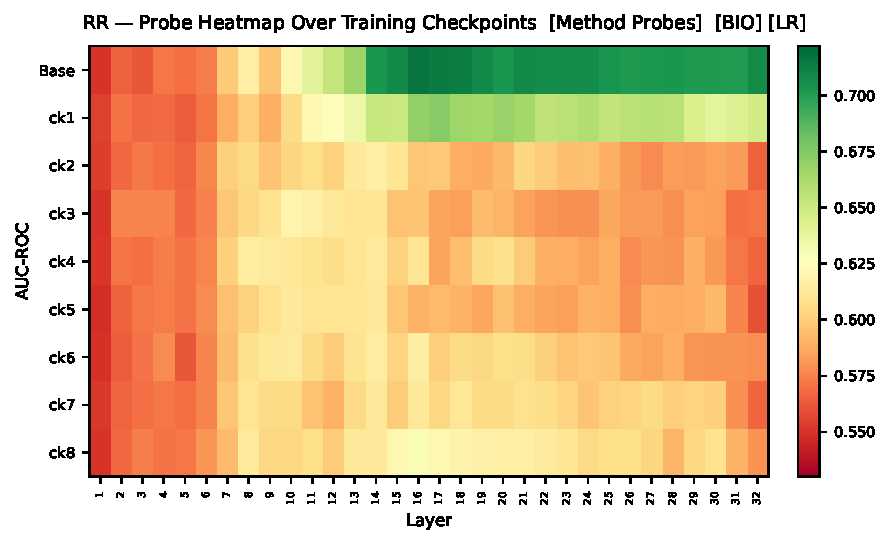
\includegraphics[width=\linewidth]{imgs/heatmap_checkpoints_auc_lr_method_bio_RR.pdf}
    \caption{LR probe AUC on WMDP-bio across unlearning checkpoints (1--8) for \textbf{RR}. Rows are transformer layers (0--32); columns are checkpoints.}
    \label{fig:heatmap-rr}
\end{figure}

\begin{figure}[H]
    \centering
    \includegraphics[width=\linewidth]{imgs/heatmap_checkpoints_auc_lr_method_bio_TAR.pdf}
    \caption{LR probe AUC on WMDP-bio across unlearning checkpoints (1--8) for \textbf{TAR}. Rows are transformer layers (0--32); columns are checkpoints.}
    \label{fig:heatmap-tar}
\end{figure}

\begin{figure}[H]
    \centering
    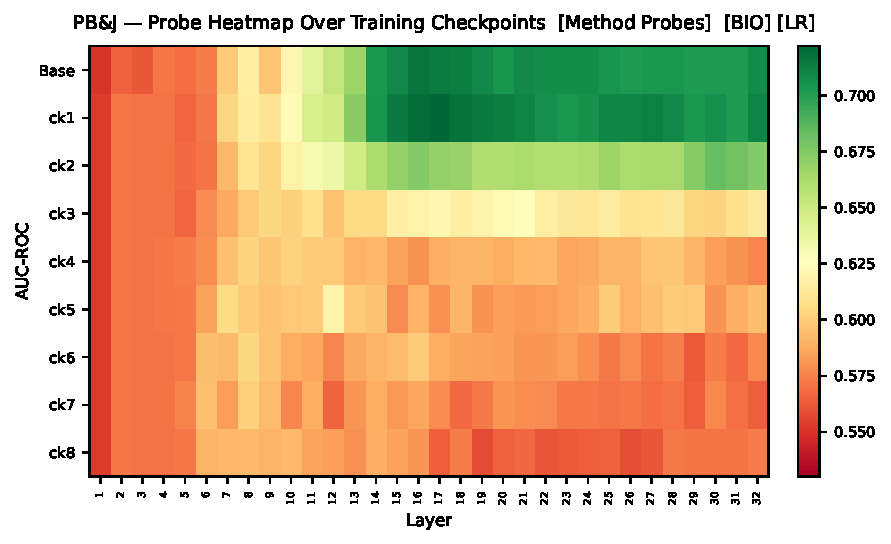
\includegraphics[width=\linewidth]{imgs/heatmap_checkpoints_auc_lr_method_bio_PB_J.pdf}
    \caption{LR probe AUC on WMDP-bio across unlearning checkpoints (1--8) for \textbf{PB\&J}. Rows are transformer layers (0--32); columns are checkpoints.}
    \label{fig:heatmap-pb-j}
\end{figure}

